\documentclass[conference]{IEEEtran}
\IEEEoverridecommandlockouts
% The preceding line is only needed to identify funding in the first footnote. If that is unneeded, please comment it out.
\usepackage{cite}
\usepackage{amsmath,amssymb,amsfonts}
\usepackage{algorithmic}
\usepackage{graphicx}
\usepackage{textcomp}
\usepackage{xcolor}
\usepackage{url}
\usepackage{hyperref}
\usepackage{pgffor}  % For the loop
\usepackage{caption} % For captions
\usepackage{float}
\usepackage{multirow}
\def\BibTeX{{\rm B\kern-.05em{\sc i\kern-.025em b}\kern-.08em
    T\kern-.1667em\lower.7ex\hbox{E}\kern-.125emX}}

% Define the folder containing the images
\newcommand*{\graphs}
{
  graphs/Local_localActionsCount_codeSize.png,
  graphs/Local_localActionsCount_contributor_count.png,
  graphs/Local_localActionsCount_created_at.png,
  graphs/Local_localActionsCount_languagesCount.png,
  graphs/Local_localActionsCount_size.png,
  graphs/Local_localActionsUsedCount_codeSize.png,
  graphs/Local_localActionsUsedCount_contributor_count.png,
  graphs/Local_localActionsUsedCount_created_at.png,
  graphs/Local_localActionsUsedCount_languagesCount.png,
  graphs/Local_localActionsUsedCount_size.png,
  graphs/Marketplace_marketActionsCount_codeSize.png,
  graphs/Marketplace_marketActionsCount_contributor_count.png,
  graphs/Marketplace_marketActionsCount_created_at.png,
  graphs/Marketplace_marketActionsCount_languagesCount.png,
  graphs/Marketplace_marketActionsCount_size.png,
  graphs/Marketplace_marketplaceActionsUsedCount_codeSize.png,
  graphs/Marketplace_marketplaceActionsUsedCount_contributor_count.png,
  graphs/Marketplace_marketplaceActionsUsedCount_created_at.png,
  graphs/Marketplace_marketplaceActionsUsedCount_languagesCount.png,
  graphs/Marketplace_marketplaceActionsUsedCount_size.png
}
\begin{document}

\title{Exploring the factors and challenges in GitHub Actions and its ecosystem\\}

\author{\IEEEauthorblockN{1\textsuperscript{st} Saif Sayed}
\IEEEauthorblockA{\textit{Department of Computer Science and Engineering} \\
\textit{University of Gothenburg}\\
Gothenburg, Sweden\\
gussayedfa@student.gu.se}
\and
\IEEEauthorblockN{2\textsuperscript{nd} Kardo Marof}
\IEEEauthorblockA{\textit{Department of Computer Science and Engineering} \\
\textit{University of Gothenburg}\\
Gothenburg, Sweden\\
gusmaroka@student.gu.se}
}

\maketitle

                                                                      %%% ABSTRACT %%%
\begin{abstract}
  Introduced in 2019, GitHub Actions offers an integrated alternative to traditional CI/CD services specifically for GitHub repositories. This deep integration enables developers to automate a wide range of software development workflows directly within the GitHub environment. Over the years, the GitHub Actions ecosystem has evolved into a mature software ecosystem, experiencing exponential growth in minutes of Actions usage. While previous studies have highlighted similarities between GitHub and package management ecosystems that distribute software libraries, our study provides an in-depth analysis of a dataset comprising 997 online posts from GitHub Discussions and Stack Overflow. These posts address prevalent issues in such ecosystems, including security, breaking changes, obsolescence, and dependency. 

  We empirically demonstrate the prevalence of these issues in GitHub Actions. Our thematic analysis on GitHub Discussion posts and Stack Overflow questions revealed that Security Vulnerability is the most prevalent issue in the GHA ecosystem, followed by Dependency Issues. Obsolescence and Breaking Changes have a similar number of occurrences. 

   Additionally, we analyzed a dataset of 4.1k GitHub repositories to examine the relationships between repository characteristics and their usage of GitHub Actions, focusing on the preference for locally maintained actions versus marketplace actions in light of ecosystem problems. Our results indicate an overall positive reliability of projects utilizing marketplace actions, with a higher correlation of marketplace actions being employed in larger and more complex projects. \\ 
 \end{abstract}

\begin{IEEEkeywords}
GHA, Action, security vulnerability, obsolescence, breaking changes, dependency issues, Local Marketplace Actions, Marketplace Actions, ecosystem, issues
\end{IEEEkeywords}

                                                                      %%% INTRODUCTION %%%
\section{Introduction}
    Continuous Integration (CI) has become an integrated part of collaborative software development and DevOps practices. CI automates the quality of code checks, tests and integration of code changes in collaborative environments. The benefits of CI brings early detection of issues, fast feedback loops, increased code quality, reduced integration risks and continuous improvements. Famous examples of CI services include Jenkins, Travis, CircleCI and GitLab CI/CD \cite{dabbish2012social}. GitHub Actions (abbreviated as GHA) was introduced to the public in 2019 as an alternative CI service for GitHub repositories. GitHub introduced its marketplace for sharing automation tools in an effort for developers to reuse workflow components \cite{saroar2023developers}. 

    The so called "Actions" refers to automated workflows triggered by specific events within a repository, including committing changes, opening pull requests, or creating new branches. These workflows streamline development processes by automating tasks and enhancing efficiency. GitHub's integration of GHA allows developers to define custom task sequences in response to events, simplifying collaboration and promoting a seamless development experience \cite{chandrasekara2021getting}. 

    The growing popularity of GHA is immense, with on average more than 20 million GitHub Action minutes used per day in 2023. This growth leads to a 169\% increase in the usage of automating tasks in public projects,  pipelines and more\cite{github2023octoverse}. Given its popularity,  the increasing usage of GHA has lead to an emergence of its own ecosystem \cite{decan2022use}.  According to Decan et al. \cite{decan2022use}, the growing ecosystem of GHA bears similarities to reusable software libraries distributed by package managers such as npm, Cargo, RubyGems, Maven and PyPI among others. Where these ecosystems are well known to suffer from variety of issues such as obsolescence, dependency issues, breaking changes and security vulnerabilities\cite{decan2022use}. The authors go on to state:\\

"\textit{The GHA ecosystem is likely to suffer from very similar issues and these issues will continue to become more important and more impactful, as the number of reusable Actions continues to grow at a rapid pace.}"\\\\
Given the concerns surrounding the GHA ecosystem, it is self-evident that developers will experience the effects of these issues.  Moreover, it's worth noting that not all Actions are available on the GitHub marketplace. Many developers create and maintain their own Actions within local repositories, without making them available on the marketplace. The authors  conducted an analysis of prevalent automation practices on GitHub and discovered that 43.9\% of repositories in their dataset reflected this behavior \cite{decan2022use}.

	Due to its novelty, there is limited understanding of the challenges faced when using GHA. Therefore,  by systematically analysing StackOverflow posts, GitHub Discussions threads, tags, and other pertinent repositories, alongside the utilisation of database queries and APIs, we aim to quantitatively  and qualitatively examine the questions, topics, and answers surrounding GHA. This endeavor not only facilitates the clarification of prevalent issues but also provides insights into potential solutions and areas requiring further research and development within the GHA landscape.\\

    Through this research, we intend to answer the following questions:\\


    \textbf{RQ1: What factors can be attributed to GitHub repositories to rely on Local Actions, as opposed to utilizing Actions available on the GitHub Marketplace?}\\

    Both Saroar et al. \cite{saroar2023developers} and Decan et al. \cite{decan2022use} observed that many repositories still prefer to use Local Actions, despite the availability of numerous open-source and reusable actions on the GitHub Marketplace. However, these studies do not investigate the exact factors or make comparisons between the two types of Actions that contribute to the differences in their usage. We selected RQ1 to measure the difference in usage between locally maintained and Marketplace Actions, and what factors attribute to these differences to reach a conclusion that can provide valuable insights into the decision-making process for designing and developing workflows. \\

 \textbf{RQ2: In what ways do the key issues encountered in GHA parallel those found in other software ecosystems?}\\

    This research question is inspired by the concerns raised by Decan \cite{decan2022use}, as previously mentioned. The objective is to compile a list of current issues prevalent in reusable software libraries distributed via package managers and draw parallels with our research findings. This comparative analysis aims to determine whether these concerns are indeed applicable to the GHA ecosystem. If similarities are found, it will aid in identifying effective solutions previously implemented in other ecosystems to address these issues. Subsequently, these solutions can be adapted for the GHA ecosystem to prevent the escalation of such problems in the future.



                                                                        %%% RELATED WORK %%%

\section{Related Work}
    After just 18 months since its official release, previous research has demonstrated a notable surge in the popularity of GHA, leading to a gradual shift away from conventional CI/CD services in GitHub repositories \cite{golzadeh2021rise}. Unlike conventional CI/CD services, GHA assists the software development processes by improving code reviews, team communication and internal repository management in addition to automating the build and test procedures of software \cite{chandrasekara2021hands}. As previously mentioned, this emerging popularity on the use of GHA and the increasing number of reusable Actions that can be found on its marketplace led GHA to be considered similar to popular reusable software libraries distributed by package managers such as npm, Cargo, RubyGems, Maven and PyPI and so on. However, this also means GHA is more likely to face similar problems that are currently encountered by these reusable libraries \cite{decan2022use}. Consequently, this would increase the chances of failure when building GitHub workflows in GitHub repositories leading to unsuccessful deployment of software packages.

    According to Decan \cite{decan2022use}, the GHA ecosystem deserves to be studied as all other reusable software ecosystems that have made progress in finding issues related to them. Since GHA is a new emerging ecosystem, there is a lack of research and studies that have been carried out to identify the challenges and issues that are encountered in GHA. The authors point out that the GHA ecosystem is exposed to similar challenges, such as obsolescence \cite{decan2018evolution} \cite{cogo2021deprecation}, dependency issues \cite{decan2019empirical} \cite{soto2021comprehensive} \cite{decan2019package}, breaking changes \cite{dietrich2019dependency}\cite{decan2018impact} and security vulnerabilities \cite{zimmermann2019small} \cite{kula2018developers}, that are encountered in well-researched ecosystems. This section aims to briefly describe some of the issues pointed out above, using findings from related literatures, that are likely to appear in GHA.

    \subsection{Obsolescence}
        Software codes are regularly updated to add features, fix bugs, etc. Sometimes functions or parts of code become deprecated meaning they are outdated and no longer used; this usually happens after a long period of time, when parts of the software code are replaced by an improved version. Generally, it is a good practice to avoid using deprecated code. Through the findings of Cogo et al. \cite{cogo2021deprecation}, deprecated code used in npm packages has shown to give rise to risks such as incompatibility between two different dependant libraries, presence/absence of features, bugs, security vulnerability and more. Cox et al. \cite{cox2015measuring} found that deprecated systems are four times more likely to suffer from security issues and backward incompatibilities than systems that are up-to-date. In the context of GHA, there is a high possibility that a significant amount of code used within the workflow is deprecated which may consequently lead to build failures.

    \subsection{Dependency Issues}
        Software systems are usually developed using pre-existing and reusable packages such as modules, components, libraries, etc \cite{decan2019empirical}\cite{soto2021comprehensive}. Consequently, this leads to a large extent of dependencies between the reused packages and the original software code. According to Dietrich et al. \cite{dietrich2019dependency}, software developers struggle to choose which versions of a given package to use and that a handful number of software systems encounter runtime version conflicts due to incompatibility with the versions of other dependant packages. Actions and workflows that depend on jobs from other Actions might fall on a similar pitfall of runtime version conflicts and possibly other dependency issues. Valenzuela-Toledo and Bergel \cite{valenzuela2022evolution} claim they have found instances of workflows where modifications were made to update the version of the tool/software being used in a particular job (e.g., Figure 1 \cite{valenzuela2022evolution}  ).

\begin{figure} [H]
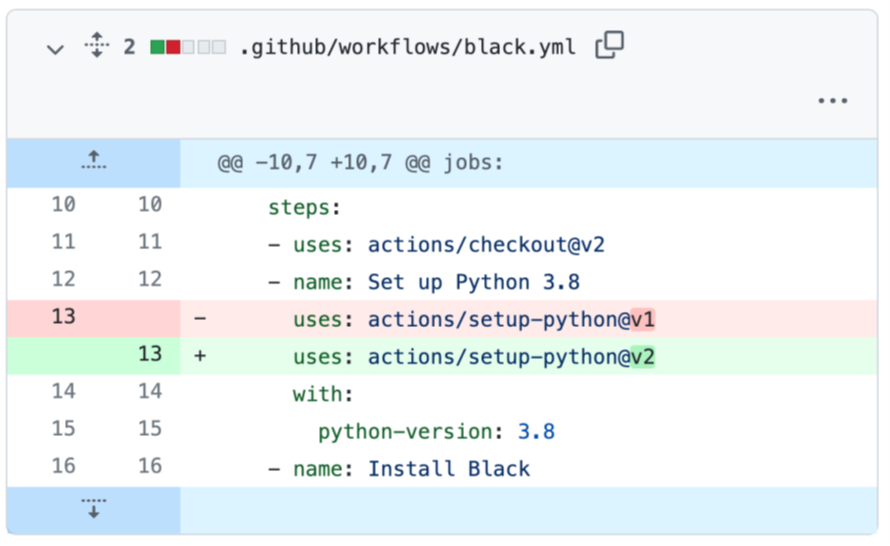
\includegraphics[width=0.5\textwidth]{Figure 1.png}
\caption{Modifying python version \cite{valenzuela2022evolution} }
\end{figure}

    \subsection{Security Vulnerabilities}
        Software that depends on open source and free reusable libraries provided by package managers like npm are more likely to be exposed to security vulnerabilities. To quote Zimmermann et al. \cite{zimmermann2019small}, they mention the following: \\

        \textit{"The open nature of npm has boosted its growth, providing over 800,000 free and reusable software packages. Unfortunately, this open nature also causes security risks, as evidenced by recent incidents of single packages that broke or attacked software running on millions of computers.”} \\\\
According to Koishybayev et al. \cite{koishybayev2022characterizing}, one example of a similar attack using the GHA ecosystem is to perform deployments based on the attacker’s code by triggering a misconfigured workflow through a new pull request. Since GHA consists of many open-source reusable Actions, workflow and GHA developers need to be extra careful on choosing what packages they depend on for building jobs. It is a good practice to depend on first-party packages and packages from trustworthy maintainers \cite{zimmermann2019small}. \\

        Saroar et al. \cite{saroar2023developers} mentions that even though the GHA platform provides a Marketplace for sharing and reusing open-source Actions, there are still many repositories that prefer to maintain their own GHA locally within their repositories. The survey analysis conducted by the authors revealed some challenges GitHub users face using the Marketplace where 7 out of 25 participants found it difficult to search for products and hard to check product quality (see Figure 2). Saroar et al. \cite{saroar2023developers} quotes one of the participants from the survey: \\

\textit{"Marketplace does not provide an effective way to filter and sort based on quality, version, contributions, etc."}\\

\begin{figure} [H]
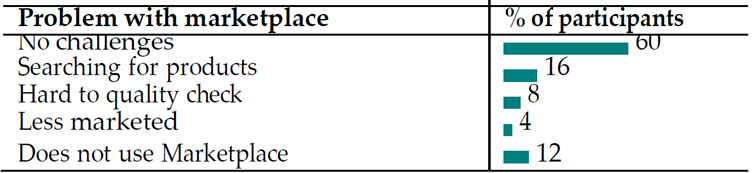
\includegraphics[width=0.5\textwidth]{Table 1.png}
\caption{Challenges found when using GitHub Marketplace \cite{saroar2023developers} }
\end{figure}

	Decan et al. \cite{decan2022use} raised concerns regarding potential issues that might be encountered by GHA, including obsolescence, dependency issues, breaking changes, and security vulnerabilities. These issues have already been faced in reusable software libraries within well-researched ecosystems. In our exploratory study, we aim to investigate whether similar problems also exist within the GHA ecosystem. Moreover, we will compile a list of specific issues from the aforementioned papers and compare our research findings on key issues in GHA with those identified in other ecosystems discussed in the literature. By doing so, we can potentially identify solutions proposed for similar issues in other ecosystems, which could offer insights into addressing the challenges encountered in GHA.

	Furthermore, our study aims to build upon the findings of Saroar et al. \cite{saroar2023developers}, identifying factors for their observations regarding the distribution of Local Actions compared to Actions from the Marketplace. While the survey conducted by the authors offers valuable insights into the challenges faced when utilizing the GitHub Marketplace, it lacks comprehensive research and comparison involving Local Actions. The primary objective of our research is to evaluate repositories' preferences in utilizing Local Actions versus Actions from the GitHub Marketplace. By doing so, we aim to identify the factors that contribute to these preferences and the resulting differences in adoption.



                                                                        %%% RESEARCH MOTHODOLOGY %%%

\section{Research Methodology}
    In this study, we aim to address the challenges developers encounter when building with GHA and to measure the extent to which locally maintained actions are utilized. In light of its ecosystem, our goal is to evaluate whether similar challenges and issues from well-researched reusable libraries can be spotted in the GHA ecosystem.

In this section, we describe the research questions we are trying to answer and the research strategies that have been implemented to facilitate our explorative study. Additionally, we would like to emphasize that we are employing different data collection and analysis methods that will be described and motivated after each research question. Our data collection process can be replicated using our scripts available in the \href{https://doi.org/10.5281/zenodo.11268782} {zenodo package}\cite{Marof2024} . Finally, we identify and explain the limitations relevant to our research and how we can mitigate them. 

    \subsection{Research questions and methodology}
        \textbf{RQ1: What factors can be attributed to GitHub repositories to rely on Local Actions, as opposed to utilizing Actions available on the GitHub Marketplace?}\\\\
 \textbf{Research Method:}  Repository Mining 

          This research question is answered by measuring similar characteristics of GitHub repositories that utilise GHA. And how these characteristics can correlate with the usage of locally maintained Actions (Local Actions). By quantitatively measuring the following characteristics, we can make an argument for whether or not the preference for using Local Actions can be tied to project size, project complexity, organization, and team size. \\
          \begin{itemize}
            \item \textbf{Repository size:} Repository size in bytes. This includes all files such as source code, artifacts, documentation, data, etc.
            \item \textbf{Number of contributors:} How many developers have contributed to the repository. May indicate the size of the team working on the project.
            \item	\textbf{Number of programming languages used:} How many types of programming langugaes used within the project. May indicate a higher complexity of the project.
            \item \textbf{Date of repository creation:} Date of creation. May indicate trends and cultral shifts.
            \item \textbf{Size of source code:} Only the amount of source code available in bytes. May also indicate a higher complexity of the project. \\
          \end{itemize}
          
          \subsubsection{\textbf{Data Collection}}
            The study utilizes python scripts\cite{Marof2024}  to collect and store repositories using GHA. Workflow files are fetched from all the stored GitHub repositories using the GitHub API.  The workflow files are then parsed, with each line iterated, to search for the $uses:$ keyword and check whether the reference of the Action matches that of a Marketplace Action or a Local Action. To distinguish between the patterns, we check whether the Action reference matches the pattern $/.github*$ or $*.yml$ or $*.yaml$. If it does, we determine that it is a Local Action, due to the reason that Local Actions are called from a file path that reside within the $/.github*$ folder or end with the file extention $*.yml$ or $*.yaml$.

Similarly, for Marketplace Actions we check whether the Action reference contains the symbol $@$. If it does, we can determine that it is a Marketplace Action. However, an important note here is that developers and organizations may have references of Actions that are locally maintained by themselves, but the Actions are kept in other repositories. In this case, an $@$ symbol is also present. To fully determine if an Action is indeed a Marketplace Action in this scenario, we have applied a step to verify that the owner of the repository and the owner of the Action do not match. The owner verification step can help with the accuracy of the measurement, because in certain cases the pattern in which the Action is called can be nuanced and can lead to false positives in measuring the amount of Marketplace Actions.
 
            To avoid redundancy, whenever an Action name is parsed out, that record is saved into a set with an attribute called $times.used$. If the same action is referenced elsewhere in Workflow, we increase $times.used$ by one data point. The $times.used$ attribute can allow us to measure the resuability of an Action within a repository workflow.\\

          \subsubsection{\textbf{Data Analysis}}
            In the analysis we have taken a quantitative approach to measure the correlations between repository characteristics and the number of Actions. In order to ensure an accurate understanding of what factors are correlated to relying on Local Actions more, the same quantitative analysis has been conducted for both Local and Marketplace Actions. We have used the Spearman correlation coefficient (SCC) method to measure the correlations coefficient of each of the repository characteristics alongside the number of Local and Marketplace Actions available and referenced. The Spearman rank correlation coefficient, \(\rho\), is a measure of the strength and direction of the association between two ranked variables. It is calculated using the formula:

            \begin{equation}
            \rho = 1 - \frac{6 \sum d_i^2}{n(n^2 - 1)}
            \end{equation}
where \(d_i\) is the difference between the ranks of each pair of observations and \(n\) is the number of observations. This non-parametric measure is used to assess how well the relationship between two variables can be described using a monotonic function.            

	We have then compared the results of these measurements to indicate if the preference for selecting Local Actions increases more than Marketplace Actions alongside any of the repository characteristics.

            Owner based frequency measurement for the amount of Local Actions available per owner can also help with determining whether big organizations lean more towards developing in-house Actions. For this analysis we have aggregated the results of Local Actions available per repository and categorized them per owner. The results from this analysis can indicate whether bigger organizations have a higher frequency in utilizing Local Actions more. \\

        \textbf{RQ2: In what ways do the key issues encountered in GHA parallel those found in other software ecosystems?}\\\\
            \textbf{Research Method:} Repository Mining

            We are already aware of the key problems encountered in other ecosystems. Our goal is to identify similar challenges and/or issues within the GHA ecosystem and evaluate the prevalence of these problems.

            To address RQ2, we plan to carry out repository mining. Through repository mining, we can collect vast amounts of data from relevant online posts related to GHA. We can also automate the process of mining data by developing scripts\cite{Marof2024}  and easing the process of going through multiple repositories \cite{chaturvedi2013tools}.\\

            \subsubsection{\textbf{Data Collection}}
We begin our data collection process by compiling a list of both general and specific issues faced by various ecosystems, such as npm, Maven, Cargo, RubyGems, etc., as identified through related literature. These issues fall into four key areas: (i) Security Vulnerability, (ii) Obsolescence, (iii) Breaking Changes, and (iv) Dependency Issues, which are commonly encountered in ecosystems with a large number of reusable, open-source packages. \textbf{Table~\ref{tab:compiled_issues}} presents our finalized compilation of these issues along with their referenced literature. The $Id$ column is used to refer to specific issues when comparing our findings in GHA with those in other ecosystems.\\
\begin{table*}[!t]
    \caption{Compilation of issues from other ecosystems.}
    \label{tab:compiled_issues}
    \begin{tabular}{|p{3cm}|p{14cm}|}
        \hline
        \textbf{Problem Id} & \textbf{Issues encountered in other ecosystems} \\
        \hline
        \multirow{8}{*}{\textbf{1.} Security vulnerability} &  \textbf{1.1.} Found atleast one library with a vulnerability in Node.js and Ruby packages \cite{decan2018impact}.\\
							&  \textbf{1.2.} Security bug in the OpenSSL cryptography library \cite{decan2018impact} with a simple programming mistake. \\							&  \textbf{Consequences:}\\
							&  (i) Memory Access by anyone on the internet.\\
							&  (ii) Many trusted servers were exposed. \\
							&  \textbf{Solution:}\\
							&  (i) Monitoring  dependencies of packages and trigger alerts when vulnerabilities are detected.\\
							&  (ii) Bounty hunting programs (lack of automated tools to assess security vulnerability in dependency networks).\\
							&  \textbf{1.3.} Spread of vulnerability  through vulnerable packages \cite{decan2018impact}.  \\
							&  \textbf{1.4.} Challenging fixes due to semantic versioning and dependency constraint \cite{decan2018impact}.\\
							&  \textbf{1.5.} Open nature of npm that caused its single packages to break/attack software running on millions of computers \cite{zimmermann2019small}.\\
							&  \textbf{1.6.} Electron distributed by npm on Windows platform affected other external software such as Skype,  slack due to exposure \cite{decan2018impact}. \\
							&  \textbf{1.7.} Security issues and single point of failure from unmaintained packages in npm \cite{zimmermann2019small}.\\
							&  \textbf{1.8.} Access to credentials for the eslint-scope package from npm  caused the attacker to release a malicious version of it for download \cite{zimmermann2019small}.  \\			
        \hline
        \multirow{7}{*}{\textbf{2.} Obsolescence} &\textbf{2.1.} 81.5\% of open-source software systems studied had outdated dependencies \cite{decan2018impact}.  \\
					      & \textbf{2.2.} Depending on outdated packages 4 times likely to  be expose to security vulnerability \cite{cox2015measuring}.  \\	
					      & \textbf{2.3.} Deprecated code in npm packages has shown to give rise to risks such as incompatibility between two different dependant libraries, presence/absence of features, bugs, security vulnerability and more \cite{cogo2021deprecation}. \\
					      & \textbf{2.4.} Technical lag in npm where package dependencies are outdated \cite{decan2018evolution}.  \\
					      & \textbf{Solution:} Dependency management tools to notify when newer versions of dependencies are released.\\
					      & \textbf{2.5.} Strict dependency constraints in npm packages that doesn’t allow dependencies to be updated to newer versions \cite{decan2018evolution}.  \\
					      & \textbf{2.6.} Security vulnerabilities found in 98\% of libraries in the Android ecosystem using outdated versions \cite{decan2018evolution}. These can easily be fixed just by changing the version. \\
					      & \textbf{2.7.} Transitive adoption of deprecated releases in npm that are hard to capture \cite{cogo2021deprecation}.  \\
        \hline
        \multirow{6}{*}{\textbf{3.} Breaking changes} & \textbf{3.1.} Limitations due to semantic versioning and dependency constraint \cite{decan2018impact}. \\
						    & \textbf{3.2.} Inclusion of versions that contain backward incompatible in the dependency constraint \cite{decan2018impact}.  \\
						    &\textbf{3.3.} Backward incompatibility risk when depending on outdated modules \cite{decan2018impact}.  \\
						    & \textbf{3.4.} Left-pad incident in npm: removal of the left-pad library caused many dependent packages to become unavailable \cite{zimmermann2019small}. \\
						    & \textbf{3.5.} Loose dependency constraint allows backward incompatibility in CRAN, RubyGems package \cite{decan2018evolution}.\\
						   & \textbf{3.6.}  Breaking changes in Maven ecosystem due to deprecation \cite{decan2018evolution}.\\
       \hline
        \multirow{7}{*}{\textbf{4.} Dependency issues} & \textbf{4.1.} Software systems depending on the vulnerable versions of the  OpenSSL software \cite{decan2018impact} . Same consequences and solution as in \textbf{Problem Id 1.2.}\\
						     & \textbf{4.2.} Removing package dependency to avoid spread of bugs \cite{decan2018impact} . \\	
						     & \textbf{4.3.} Limitations due to semantic versioning and dependency constraint \cite{decan2018impact}.\\
						     & \textbf{4.4.} Changing back to an earlier version or a recent version that doesn’t contain bug \cite{decan2018impact}  .\\
						     & \textbf{4.5.} Runtime conflicts due to incompatibility with
the versions of other dependant packages \cite{dietrich2019dependency}.
 \\
						     & \textbf{4.6.} Left-pad incident in npm: removal of the left-pad library caused many dependent packages to become unavailable \cite{zimmermann2019small}.  \\
						     & \textbf{4.7.} High number of transitive dependencies in npm  being reused \cite{zimmermann2019small}.  \\
        \hline
    \end{tabular}
\end{table*}
             Repository mining is conducted by utilizing APIs and database queries to collect relevant data from Stack Overflow, GitHub Discussions, and other pertinent repositories. To collect data from GitHub Discussions, we use the GraphQL API in our scripts \cite{Marof2024} to extract and store relevant discussion posts in JSON format. Specifically, we search for all discussion posts that contain the query string "GitHub Actions". The scripts then target the four key issues mentioned above and their synonyms to filter posts that may contain the relevant problems. \textbf{Table~\ref{tab:related_keywords}} documents the four key issues and their corresponding synonyms, along with related keywords used for filtering. \\
  \begin{table}[H]
          \centering
          \caption{Key issues and related keywords used for filtering.}
          \label{tab:related_keywords}
	\hspace{5cm}
          \begin{tabular}{|c|c|}
              \hline
              \textbf{Key issues} & \textbf{Synonyms and related keywords} \\
              \hline
              Security vulnerability & \parbox[t]{5.5cm}{risk*, vulnerab*, exploit*, attack*, malicious, harmful, unmaintained, secur*, steal, credential*, secret*, inject*, access*, expose*, compromise*, trust*, untrust*, change*, threat*, package*, librar*, bug*,  version*, affect*\\}  \\
             \hline
             Obsolescence & \parbox[t]{5.5cm}{outdated*, legacy, deprecat*, obsolete, unmaintained, obsolescence, update*, up-to-date, out-of-date, package*, librar*, version*, affect*, technical lag, latest, old*, depend*\\}  \\
              \hline
              Breaking changes & \parbox[t]{5.5cm}{breaking change*,  backward, compatib*, package*, librar*, version*, affect*, mismatch, conflict, depend*\\} \\
              \hline
              Dependency issues &  \parbox[t]{5.5cm}{conflict, mismatch, package*, version*, incompatib*, compatib*, transitive depend*, rely*, depend*, librar*, affect*, direct\\}  \\
              \hline
          \end{tabular}
\end{table}
                A similar approach is used to collect questions from Stackoverflow using the Stackoverflow API. Our scripts searches for all the questions that are tagged $GitHub-Actions$ and then targets the aforementioned issues and their synonyms. The discussion posts and questions have been analyzed manually, and conclusions about the problems are drawn.\\

            \subsubsection{\textbf{Data Analysis}}
                In our data analysis approach, we employed repository mining techniques to analyze patterns and trends in Stack Overflow posts and GitHub Discussion threads obtained through APIs and database queries. During our data collection process, we filtered posts and questions using key issues and their related keywords as search targets. For each filtered posts and questions, we compiled a list of keywords that appeared in them for each key issue. Then, for each key issue, we filtered the posts and questions that contained more than one keyword. We conducted this procedure independently for each key issue to prevent mixing posts and questions from different key issues.

               After obtaining the filtered data with multiple related keywords, we manually inspected the titles and corresponding list of keywords that appeared in each instance to determine their relevancy for our thematic analysis. For instance, a GitHub Discussion post titled “Organization-wide Environments and Environment Secrets" included keywords such as 'attack', 'credential', 'secret', and 'access', indicating its relevance to the key issue “Security Vulnerability". We assessed the relevance of each post and question manually and restricted the number of posts for our thematic analysis.

	Once we finalized our list of posts and questions, we conducted our thematic analysis using the “Braun \& Clark (2006)” method. This method helps organize and elaborate on data efficiently and is effective in identifying patterns and trends within the research topic.

	To exemplify our thematic analysis process, consider the following data extract from a GitHub Discussion thread:\\\\
“\textit{Considering how organization-level secrets are indirectly available to all users with write access, environments are the only way to protect sensitive secrets from attacks originating inside the organization (e.g., stolen credentials). Without organization-wide environments, protecting sensitive secrets across multiple repositories is a huge pain.}”\\\\
This statement corresponds to two codes defined in our Codebook in \textbf{Appendix B}, namely V-A and V-S, both related to the top-level theme Vulnerability (V). V-A represents the sub-theme \texttt{Access Vulnerability}, and V-S represents the sub-theme \texttt{Solution Vulnerability}. The first sentence relates to \texttt{Access Vulnerability} as it involves attacks by users with write access. The second sentence pertains to a solution for the vulnerability, where the use of organization environments can potentially protect sensitive secrets. Overall, our approach aimed to provide a comprehensive understanding of the challenges in the GHA ecosystem parallel to other software ecosystems.\\

These methods ensure a systematic approach to address each research question effectively.\\


    \subsection{Threats to Validity}
        In this section, we discuss the limitations and threats to
        validity and how we can mitigate them.\\

        \textbf{External Validity:} Since our repository mining procedure is supposed to collect data from diverse GitHub repositories with different implementation of workflows, programming languages and size of the project, the results we obtain might differ depending on these factors and our findings can not be generalized for all types of GitHub projects. However, it is possible to group the projects based on their size, programming language, etc. After grouping the projects, we could try to analyse data from each group and identify a common trend between the results to generalize our findings.\\

	\textbf{Construct Validity:} Our thematic analysis may encounter issues related to subjectivity and biases, as it heavily relies on the interpretation of the researcher. Personal biases and preconceptions about the research topic can influence how the data is coded and themes are identified. To address this concern, one of us developed the codes, while the other person validated them to ensure that thematic coding remains free from personal biases and preconceptions.

	Our data collection process is also constrained by the target keywords we used to filter our data. We can only capture posts that contain the specified keywords, and the effectiveness of our data collection depends on how well we define these keywords to capture relevant posts and questions. To mitigate these risks, we ensured that the keywords were not redundant and captured multiple forms of the same keyword. For instance, 'dependency' might have other forms such as 'depend', 'dependencies', and 'dependable'. To capture all these variations, we used 'depend*' with a wildcard '*' to include all relevant forms of the keyword 'dependency'.

							    	      %%%RESULTS%%%

\section{Results}

  \subsection{RQ1}
      For RQ1, after collecting data across 4166 GitHub repositories that were on the top one-thousand list of popular repositories for the years throughout 2020, 2021, 2022, 2023 and 2024, we applied a filter to dismiss repositories that did not use any Actions. The number of repositries reduced to 1754. 

      In these repositories, Marketplace Actions consisted of 92.64\% of the total Actions, while the remaining 7.36\% consisted of Local Actions. And when analysing the number of times each Action was referenced in other parts of the workflow, we found that the result was quite similar with 92.62\% for Marketplace Actions and 7.38\% for Local Actions.

	Data on number of different programming languages, repository size, number of contributors, date of repository creation and bytes of source code were also collected in order to see if there were any correlations between these repository attributes and the amount of Marketplace or Local Actions used or referenced. Table \ref{tab:correlation_results} demonstrates the results of the correlations, categorized as Marketplace Actions and Local Actions. The number of elements in set $N$ is denoted by $|N|$, similarly for set $M$. The graphs for these comparisons are available in \textbf{Appendix A}.\\
      \begin{table}[H]
          \centering
          \caption{Spearman Correlation Coefficients between Repository Characteristics and GHA}
          \label{tab:correlation_results}
          \hspace{-1cm}
          \begin{tabular}{|l|l|r|}
              \hline
              \textbf{Repository Characteristic} & \textbf{GitHub Action Type} & \textbf{(\(\rho\))} \\
              \hline
              Source Code size (bytes) & $|M|$ Local Actions & 0.23 \\
              \hline
              $|N|$ contributors &  $|M|$ Local Actions & 0.21 \\
              \hline
              Repo created (Unix timestamp) &  $|M|$ Local Actions & -0.11 \\
              \hline
              $|N|$ programming languages & $|M|$ Local Actions & 0.16 \\
              \hline
              Repository size (bytes) & $|M|$ Local Actions & 0.20 \\
              \hline
              Source Code size (bytes) & $|M|$ Local Actions referenced & 0.24 \\
              \hline
              $|N|$ contributors  & $|M|$ Local Actions referenced & 0.17 \\
              \hline
              Repo created (Unix timestamp) & $|M|$ Local Actions referenced & -0.14 \\
              \hline
              $|N|$ programming languages & $|M|$ Local Actions referenced & 0.23 \\
              \hline
              Repository size (bytes) & $|M|$ Local Actions referenced & 0.21 \\
              \hline
              Source Code size (bytes) & $|M|$ Marketplace Actions & 0.33 \\
              \hline
              $|N|$ contributors & $|M|$ Marketplace Actions & 0.30 \\
              \hline
              Repo created (Unix timestamp) & $|M|$ Marketplace Actions & -0.10 \\
              \hline
              $|N|$ programming languages & $|M|$ Marketplace Actions & 0.38 \\
              \hline
              Repository size (bytes) & $|M|$ Marketplace Actions & 0.27 \\
              \hline
              Source Code size (bytes) & $|M|$ Marketplace Actions referenced & 0.40 \\
              \hline
              $|N|$ contributors & $|M|$ Marketplace Actions referenced & 0.37 \\
              \hline
              Repo created (Unix timestamp) & $|M|$ Marketplace Actions referenced & -0.17 \\
              \hline
              $|N|$ programming languages & $|M|$ Marketplace Actions referenced & 0.41 \\
              \hline
              Repository size (bytes) & $|M|$ Marketplace Actions referenced & 0.30 \\
              \hline
          \end{tabular}
      \end{table}
      
      \subsection{Analysis of Correlations}
      
      \subsubsection{Local Actions}
      For Local Actions, several repository characteristics showed weak positive correlations:
      
      \begin{itemize}
          \item \textbf{Source Code Size:} A weak positive correlation (\(\rho = 0.23\)) was observed between the source code size and the number of Local Actions. This suggests that repositories with larger codebases tend to use more Local Actions.
          \item \textbf{Number of Contributors:} A weak positive correlation (\(\rho = 0.21\)) indicates that repositories with more contributors are slightly more likely to use Local Actions.
          \item \textbf{Repository Size:} Similar to the source code size, a weak positive correlation (\(\rho = 0.20\)) was found, reinforcing the idea that larger repositories are slightly more likely to utilise Local Actions.
          \item \textbf{Number of Programming Languages:} There is a weak positive correlation (\(\rho = 0.16\)), implying that repositories with a higher number of programming languages tend to use more Local Actions.
          \item \textbf{Repository Creation Date:} A weak negative correlation (\(\rho = -0.11\)) was observed, indicating that older repositories are less likely to use Local Actions.\\
      \end{itemize}
      
      \subsubsection{Marketplace Actions}
      Marketplace actions showed generally stronger correlations with repository characteristics compared to Local Actions:
      
      \begin{itemize}
          \item \textbf{Source Code Size:} There is a weak positive correlation (\(\rho = 0.33\)) between the source code size and the use of Marketplace Actions, indicating that larger codebases are more inclined to use Marketplace Actions.
          \item \textbf{Number of Contributors:} A weak positive correlation (\(\rho = 0.30\)) suggests that repositories with more contributors are more likely to use Marketplace Actions.
          \item \textbf{Repository Size:} A similar trend is observed with a weak positive correlation (\(\rho = 0.27\)), suggesting that larger repositories favor Marketplace Actions.
          \item \textbf{Number of Programming Languages:} The strongest positive correlation (\(\rho = 0.38\)) among all characteristics was found here, indicating a significant tendency for repositories with more programming languages to use Marketplace Actions.
          \item \textbf{Repository Creation Date:} A weak negative correlation (\(\rho = -0.10\)) indicates that older repositories are slightly less likely to use Marketplace Actions.\\
      \end{itemize}
      
      \subsubsection{Referenced Actions}
      When considering Actions referenced within repositories:
      
      \begin{itemize}
          \item \textbf{Local Actions Referenced:} The correlation coefficients for referenced Local Actions are slightly higher compared to non-referenced ones, with the highest being source code size (\(\rho = 0.24\)) and number of programming languages (\(\rho = 0.23\)).
          \item \textbf{Marketplace Actions Referenced:} The correlations are generally higher for Marketplace Actions referenced, with the number of programming languages showing a moderate positive correlation (\(\rho = 0.41\)) and source code size (\(\rho = 0.40\)).\\
      \end{itemize}

      \subsubsection{Organizational Usage of Local Actions}

      In addition to the correlation analysis, we examined the usage of Local Actions by various organizations. Table \ref{tab:org_usage} lists the top organizations based on their use of Local Actions. Notably, large organizations such as HashiCorp, Google, Microsoft, and Facebook are prominent in the usage of Local Actions, indicating a preference for maintaining their own workflows rather than relying solely on marketplace actions.
      \begin{table}[!h]
          \centering
          \caption{Top Organizations by Use of Local Actions}
          \label{tab:org_usage}
          \begin{tabular}{|l|c|}
              \hline
              \textbf{Organization} & \textbf{Number of Local Actions} \\
              \hline
              HashiCorp & 58 \\
              Datafuselabs & 46 \\
              Hugging Face & 39 \\
              NovuHQ & 26 \\
              External Secrets & 26 \\
              Google & 25 \\
              Backstage & 25 \\
              Grafana & 23 \\
              KubeVela & 22 \\
              Earthly & 20 \\
              Cilium & 19 \\
              LanceDB & 19 \\
              Firezone & 18 \\
              ZenML-io & 17 \\
              Calcom & 17 \\
              Coqui AI & 15 \\
              Microsoft & 14 \\
              Web Infra Dev & 14 \\
              Appsmithorg & 14 \\
              Anchore & 13 \\
              Rustic-rs & 13 \\
              LibJXL & 13 \\
              Anuraghazra & 12 \\
              Vercel & 12 \\
              Haiibo & 12 \\
              Bitnami & 11 \\
              Chroma Core & 11 \\
              MartinVonz & 11 \\
              DataDog & 11 \\
              Apache & 11 \\
              Kafbat & 10 \\
              Lienol & 10 \\
              Mandiant & 10 \\
              Argilla-io & 10 \\
              CloudQuery & 10 \\
              OpenTofu & 10 \\
              Alibaba & 9 \\
              Keiyoushi & 9 \\
              Sigstore & 9 \\
              DeterminateSystems & 9 \\
              Kiddin9 & 9 \\
              RustDesk & 9 \\
              Techno Tim & 9 \\
              Facebook & 9 \\
              Lucidrains & 9 \\
              Zitadel & 9 \\
              JupyterLite & 8 \\
              \hline
          \end{tabular}
      \end{table}
  \subsection{RQ2}
Our original dataset, collected through mining software repositories, comprised 997 GitHub discussion posts containing the query string "GitHub Actions" and 100 Stack Overflow questions tagged "GitHub Actions." By filtering this data using the key issues and their related keywords, we were able to collect and group posts and questions related to each key issue. We ended up with 101 posts and questions for the key issue of \textit{Security Vulnerability}, 80 posts and questions for \textit{Obsolescence}, 51 posts and questions for \textit{Breaking Changes}, and 75 posts and questions for \textit{Dependency Issues}. Since we also collected a list of target keywords that appeared in each post and question during the filtering process, we were able to narrow down the number of posts and questions needed for our thematic process. Using these lists of keywords, along with their corresponding post/question titles, we manually determined which of the collected posts and questions were relevant. \textbf{Table~\ref{tab:number_data}} shows the finalized number of posts and questions we used to perform our thematic analysis.
\begin{table}[H]
\centering
\caption{Finalised number of posts and questions.}
\label{tab:number_data}
\begin{tabular}{|c|c|c|}
  \hline
  \textbf{Key issues} & \textbf{Posts}  & \textbf{Questions} \\
  \hline
  \hline
    Security vulnerability & 16 &  2  \\
  \hline
  \hline
   Dependency changes & 10 & 6  \\
  \hline
  \hline
   Breaking Changes & 12 & 1 \\
  \hline
  \hline
   Obsolescence & 10  & 1 \\
  \hline
\end{tabular}
\end{table}

Our thematic analysis of these posts revealed that \texttt{Security Vulnerability} is the most prevalent issue in GHA ecosystem among the four key issues. This is followed by \texttt{Dependency Issues}, while both \texttt{Obsolescence} and \texttt{Breaking Changes} appear with a similar number of occurrences. The codebook, which contains our codes and themes derived from thematic analysis, is outlined in \textbf{Appendix B}. We have included results for each of the key issues and how they compare to other ecosystems in the following subsections.
\subsection*{\textbf{Security Vulnerability}}
\textbf{Related issues from other ecosystems:} 1.1., 1.2., 1.5., 1.6., 1.8. in \textbf{Table~\ref{tab:compiled_issues}}.\\

	For this key issue, our thematic analysis identified 11 occurrences of the top-level theme \texttt{Security Vulnerability}, with 8 of them related to the sub-theme \texttt{Access Vulnerability} and 3 related to the sub-theme \texttt{Attacks and Injections}. Additionally, there were 3 occurrences of the theme \texttt{Vulnerability Solution}.

	There were numerous GitHub Discussion posts and Stack Overflow questions corresponding to the theme of \texttt{Access Vulnerability}, although some had been resolved. One notable example was the absence of a feature for having \texttt{Organization Environments}, which could potentially enable malicious attacks such as stealing credentials and sensitive secrets by allowing all users within the organization with write access to perform such actions \cite{philomory2024}. However, we also identified a feature in the GHA ecosystem that prevents Actions from automatically pushing changes to protected branches, thereby mitigating the risk of anyone with write access pushing malicious code to protected branches\cite{robozevel2024}. Another similar, resolved issue involved building Actions upon the creation of tags, where environments couldn't be securely used, potentially allowing anyone with write access to bypass protection rules when creating protected tags \cite{WolfspiritM2024}. Such issues related to write access can lead to unwanted consequences, as seen in \textbf{Problem ID 1.8.} from \textbf{Table~\ref{tab:compiled_issues}}, where an attacker released a malicious version of the eslint-scope package in the npm ecosystem by gaining access to its credentials.

	\texttt{Attacks and Injections} emerged as a theme where we encountered an actual attack on the GHA ecosystem, specifically a Crypto-mining attack, where a GitHub user triggered the execution of malicious code through a pull request, allowing crypto-mining in the victim's GitHub Actions. Our analysis revealed that GHA employees swiftly responded to such occurrences and took countermeasures against them. However, some users blamed the attack on the GHA ecosystem for allowing anyone on the internet to create a free, anonymous account and trigger a pull request to any public repositories \cite{thibaultduponchelle2024}. Similar attacks using malicious code in other ecosystems can be observed in \textbf{Problem IDs 1.2, 1.5, and 1.8} from \textbf{Table~\ref{tab:compiled_issues}}. One exposed security vulnerability discovered in the GitHub Actions runner was the allowance of injecting environment variables and paths in workflows that log untrusted data to std:out. A potential consequence of this vulnerability is the introduction or modification of environment variables without the approval of the workflow author \cite{DaanDeMeyer2024}.
\subsection*{\textbf{Obsolescence}}
\textbf{Related issues from other ecosystems:} 2.1., 2.3., 2.4. in \textbf{Table~\ref{tab:compiled_issues}}.\\

	For this key issue, our thematic analysis identified 3 occurrences of the top-level theme \texttt{Obsolescence}, with 2 of them related to the sub-theme \texttt{Deprecated Versions} and 1 related to the sub-theme \texttt{Usage Of Older Actions}. Additionally, there were 2  occurrences of the theme \texttt{Obsolescence Solution}.

	The compiled codes for the theme \texttt{Deprecated Versions} corresponded to Actions that depended on deprecated versions of packages. For example, this particular version of "Xcode 11.2.1" was not supported in GitHub Actions \cite{sinoru2024}. Another issue was found in the "actions/upload-artifacts" Action, where the workflow file relied on an outdated and deprecated version that no longer supported globbing \cite{graysuit2024}. The suggested fix for this issue was to update the Action to a newer version. These issues are similar to general problems faced in other ecosystems and align with \textbf{Problem IDs 2.3. and 2.4.}, where deprecated code or packages in npm result in technical lag and functionality issues. One solution mentioned in \textbf{Problem ID 2.4.} was the introduction of Dependency management tools that can notify users when newer versions of a package are released.

	In the theme \texttt{Usage of Older Actions}, we also found a problem where a GitHub user removed a deprecated workflow file and replaced it with a newer one. However, even after removing the deprecated workflow file, the Action remained in the Action list, meaning the old workflow would still be triggered during events. One suggested solution was to remove all associated jobs with the Action, but this solution was not scalable \cite{ryanvanderpol2024}. This issue is also related to \textbf{Problem ID 2.4.}, where deprecated code in npm resulted in bugs among other problems.
\subsection*{\textbf{Breaking changes}}
\textbf{Related issues from other ecosystems:} 3.4., 3.6. in \textbf{Table~\ref{tab:compiled_issues}}.\\

	For this key issue, our thematic analysis identified 4 occurrences of the only  top-level theme \texttt{Breaking changes}.\\
In the theme \texttt{Breaking Changes}, we included the codes where a single change caused a series of issues that disrupted the usual workflow. One such issue occurred was when GitHub rolled out a security patch that limited code deployment to production by creating a tag, which in turn disabled protected environments. This deliberate decision, made until the bug was fixed, was referred to as \textbf{Security of Breaking Changes} by a GitHub user \cite{WolfspiritM2024}. Another unresolved problem found in a discussion post involved the sudden failure of a user's workflow, causing a collection of modules to fail to push packages to the GitHub Maven registry \cite{lukas-krecan2024}.

	We identified two additional issues related to breaking changes. One involved Dependabot, a GitHub Action bot, which started behaving erratically by reporting unusual dependency update PR changes, resulting in false positives. The root cause was traced to the GitHub Registry processing the metadata of gemspec packages and incorrectly tagging development package dependencies as runtime\_development dependencies \cite{nbibler2024}. The final observation in this theme was GitHub's introduction of a new mechanism that gated pull requests until all workflows were executed and passed. This change affected some users by rendering a "cached" version of the pull request, leaving the workflows pending \cite{tuves2024}.

	These issues are mostly related to \textbf{Problem ID 3.4} and share similarities in the consequences of breaking changes from \textbf{Problem ID 3.6}. In \textbf{Problem ID 3.4}, an incident is described where the removal of the Left-pad library in npm caused several dependent packages to become unavailable and resulted in breaking changes.
\subsection*{\textbf{Dependency issues}}
\textbf{Related issues from other ecosystems:} 4.5., 4.6., 4.7. in \textbf{Table~\ref{tab:compiled_issues}}.\\

	For this key issue, our thematic analysis identified 5 occurrences of the top-level theme \texttt{Dependency Issues}, with 4 of them related to the sub-theme \texttt{Direct Dependency} and 1 related to the sub-theme \texttt{Transitive Dependency}.

	In the theme \texttt{Direct Dependency}, our findings revealed two problems related to jobs being directly dependent on other jobs. One issue was that a failed job is bound to fail again during a re-run if any of its dependent jobs uses a reusable workflow. This occurs because re-running a failed job also triggers its dependent jobs to re-run, which cancels the in-process runs of those dependent jobs \cite{gvanrossum2024}. The second related problem involved dependency between two sequential jobs, such as a build and a test job, where the test job depends on the status of the build job. If the build job fails, the test job will not run \cite{hugomg2024}.

	Additional issues in this theme were related to package dependencies in Maven and GitHub Action bots. A GitHub user encountered a problem where they were unable to build their project using GitHub Actions because the Maven dependencies were not resolvable, and none of the Gradle versions could resolve the Maven dependency. This issue remained unsolved \cite{kxuenvoy2024}. Another problem, also mentioned in the \texttt{Breaking Changes} theme, involved the GitHub registry incorrectly tagging development package dependencies as runtime\_development dependencies instead of development dependencies \cite{nbibler2024}.

	In the theme \texttt{Transitive Dependency}, we collected issues with dependencies that are not directly visible to the user but can cause GitHub Actions to fail. Our observation noted that the GitHub user did not find any packages causing direct issues for the Action to fail. However, they discovered a fourth-tier dependency that caused the error. This particular issue aligns with \textbf{Problem ID 4.7.}, where a high number of transitive dependencies were being reused in npm, which was problematic\cite{hugomg22024}.
							    	      %%%CONCLUSION%%%
\section{Discussion}
	In this section, we delve into our findings for each research question by presenting insights derived from the results and our own interpretation.\\

\subsubsection{\textbf{RQ1}} The results indicate that certain repository characteristics, such as source code size, number of contributors, and number of programming languages, are positively correlated with the usage of GHA, whether locally maintained or from the marketplace. The stronger correlations for Marketplace Actions suggest that repositories with more complexity and collaboration tend to leverage Marketplace Actions more frequently. Conversely, the weak negative correlations with repository creation date suggest that newer repositories are more inclined to adopt both types of actions, potentially reflecting evolving practices and the increasing availability of GHA over time.

      In conclusion, the analysis provides insights into how various repository characteristics influence the adoption and referencing of GHA, highlighting trends that could inform best practices for repository management and automation strategy. Currently, the usage of Marketplace Actions prove to be more dominant across repositories, which may be due to the reliability and stability of the GHA ecosystem.\\

\subsubsection{\textbf{RQ2}} The results addressed concerns raised by Decan et al. \cite{decan2022use} regarding challenges exposed to the GHA ecosystem, particularly surrounding the four key issues of Obsolescence, Security Vulnerability, Breaking Changes, and Dependency Issues, which are prevalent in other ecosystems as listed in \textbf{Table~\ref{tab:compiled_issues}}. However, our findings indicated fewer or less severe problems compared to those in other ecosystems. Notably, our findings did not align with all the Problem IDs in \textbf{Table~\ref{tab:compiled_issues}}, such as issues related to semantic versioning and dependency constraints commonly observed in other ecosystems. We attribute this discrepancy to the effective maintenance of the GHA ecosystem by administrators.

	During our data analysis, we observed that GitHub Discussion posts are regularly monitored by admins, leading to immediate resolution of reported issues. In one instance, we found that attacks exploiting the GHA ecosystem are addressed immediately, even before being reported. Furthermore, additional features are developed to address concerns raised by GitHub users, which may involve bugs, security vulnerabilities, deprecated package versions, and dependency issues.
\section{Conclusion}
	In conclusion, the results of this study demonstrate that the GHA ecosystem is currently a stable and reliable environment for developers. While issues similar to those in other software ecosystems do exist, their impact appears to be less significant. The reliance on locally maintained actions is lower than on marketplace actions, indicating a high level of dependency and trust in the ecosystem-provided Actions. Although the relative novelty of the ecosystem might contribute to the lesser severity of these issues, further investigation is needed to determine if the current stability and scalability of GHA will be sustained in the long term.

\section{Future work}
	We acknowledge the potential for further research based on our findings. In RQ1, we conducted quantitative data analysis across numerous software repositories to gauge the reliance on Local Marketplace Actions. While our initial intention was to complement this with qualitative data analysis using surveys and mining GitHub discussions and Stack Overflow posts, time constraints led us to focus solely on quantitative analysis. Future studies could delve into qualitative data analysis to explore developers' preferences regarding action types and the challenges they encounter, thus reinforcing the credibility of our findings by comparing with quantitative results.

	Moreover, we noticed the predominance of large organizations in the use of Local Actions may be attributed to concerns over security risks and dependency issues associated with marketplace actions. Larger organizations might prefer to maintain control over their workflows to mitigate potential vulnerabilities and ensure stability. However, further investigation is needed to substantiate these claims and understand the underlying reasons behind this trend.

	In RQ2, we found fewer instances corresponding to the four key issues in GHA compared to other ecosystems, and the severity wasn't as pronounced. Our findings didn't align with several issues listed in \textbf{Table~\ref{tab:compiled_issues}}. As discussed earlier, this could be attributed to the well-maintained nature of the GHA ecosystem, with identified bugs and issues promptly addressed. However, to assert such claims, future investigations should explore how the ecosystem mitigates risks associated with the four key areas.

	Lastly, it would be pertinent and beneficial to compare the four key issues with other CIs such as Travis, CircleCI, and GitLab CI/CD, given their shared focus on automating code integration in collaborative platforms. This presents another avenue for future research.
							    %%% ACKNOWLEDGEMENT %%%

\section{Acknowledgement}
         This thesis report is the collaborative effort of Kardo Marof and Saif Sayed, under the guidance of our thesis supervisor, Linda Erlenhov. We would like to express our gratitude to our supervisor, Linda, for entrusting us with her proposed thesis topic and for providing prompt feedback to any queries we had through meetings and Slack communications. This thesis report would not have been possible without the late-night meetings and numerous cups of coffee we shared.
                                                                             %%% REFERENCES %%%
\bibliographystyle{IEEEtran}
\bibliography{references}

\appendix						           %%% APPENDICES%%%
\subsection{Graphs}
\foreach \x in \graphs
  {\begin{center} 
	\includegraphics[width=60mm]
		{\x} \bigskip 
  \end{center}}
\vspace{12cm}
\clearpage
\thispagestyle{empty}
\subsection{RQ2: CODEBOOK}
\begin{table}[h]
    \centering
    \label{tab:full-width}
    \hspace{0.5cm}
    \begin{tabular}{|p{3cm}|p{1cm}|p{1.5cm}|p{11cm}|}
        \hline
        \textbf{Theme} & \textbf{Codes}  & \textbf{Occurence}  & \textbf{Description} \\
        \hline
        Security Vulnerability & V & 11 & This theme is the top-level theme concerning all identified sub-themes related to security vulnerabilities. \\
        \hline
        Access Vulnerability & V-A & 8 & This sub-theme of vulnerability is related to attacks or occurrences due to access permissions to write and modify the system. \\
        \hline
        Vulnerability Solution & V-S & 3 & This sub-theme of vulnerability identifies suggested solutions by GitHub users for the identified vulnerability.\\
        \hline
        Attacks and Injections & V-AI & 3 & This sub-theme of vulnerability covers attacks or injections that occurred in the GHA ecosystem by using malicious or modified code. \\
        \hline
        Obsolescence & O & 3 & This theme is the top-level theme concerning all identified sub-themes related to obsolescence.\\
        \hline
        Deprecate Versions & O-DV & 2 & This sub-theme of obsolescence covers the identified issues and limitations that occurred due to the use of a deprecated version of a package. \\
        \hline
        Usage of Older Actions & O-UOA & 1& This sub-theme of obsolescence includes issues in the GitHub ecosystem that don't remove older Actions that are no longer being used. \\
        \hline
        Obsolescence Solution & O-S & 2 & This sub-theme of obsolescence includes all the code that suggests possible solutions to the identified issues. \\
        \hline
        Breaking Changes & BC & 4 & This is the only theme related to breaking changes, where a chain of issues was caused by a single change or update in the GHA ecosystem. \\
        \hline
        Dependency Issues & D & 5 & This is the top-level theme concerning all sub-themes related to dependency issues. \\	
        \hline
        Direct Dependency  & D-DD & 4 & This sub-theme of Dependency Issues was related to all identified issues caused by direct dependencies that are visible to the user. \\	
        \hline
        Transitive Dependency & D-TD & 1 & This sub-theme of Dependency Issues was related to all identified issues caused by transitive dependencies that aren’t visible to the user.\\	
        \hline
    \end{tabular}
\end{table}	
\end{document}
